Consider a 3SAT problem with m clauses $c_j$ and n variables $x_i$. For a given 3SAT we construct a congestion game and demonstrate that if in this game there exists a NE with the cost of 0 then the the 3SAT formula can be satisfied.
\bigskip

\uline{\textbf Graph construction.} Consider the following graph $G$. We introduce a node $C_j$ for every clause $c_j$ and three nodes $A_i,X_i,\neg\ X_i$ for every variable $x_i$.

We define two types of edges:

Type 1 edges: cost is 0 for $x=1$ and $1$ for $x\neq 1$: $c(x) = \mathbb 1[x\neq 1]$

Type 2 edges: cost is 0 for $x\leq m$ and $1$ for $x>m$: $c(x) = \mathbb 1 [x>m]$

Type 3 edges: cost is 0 for $x=m,x=0$ and $1$ otherwise: $c(x) = 1- \mathbb 1 [x\neq0]\mathbb 1 [x\neq m]$

Nodes $C_j$ are connected to the source with type 1 edges. Variable node $X_i$ ($\neg\ X_i$) are connected to clause node $C_j$ if $x_i$ is in clause $c_j$ (if $\neg x_i$ is in $c_j$) with edges of cost 0.  Variable nodes $X_i,\ \neg X_i$ are also connected to the $A_i$ node with type 3 edges and to the sink with type 2 edges. Nodes $A_i$ are connected to the source with type 2 edges.

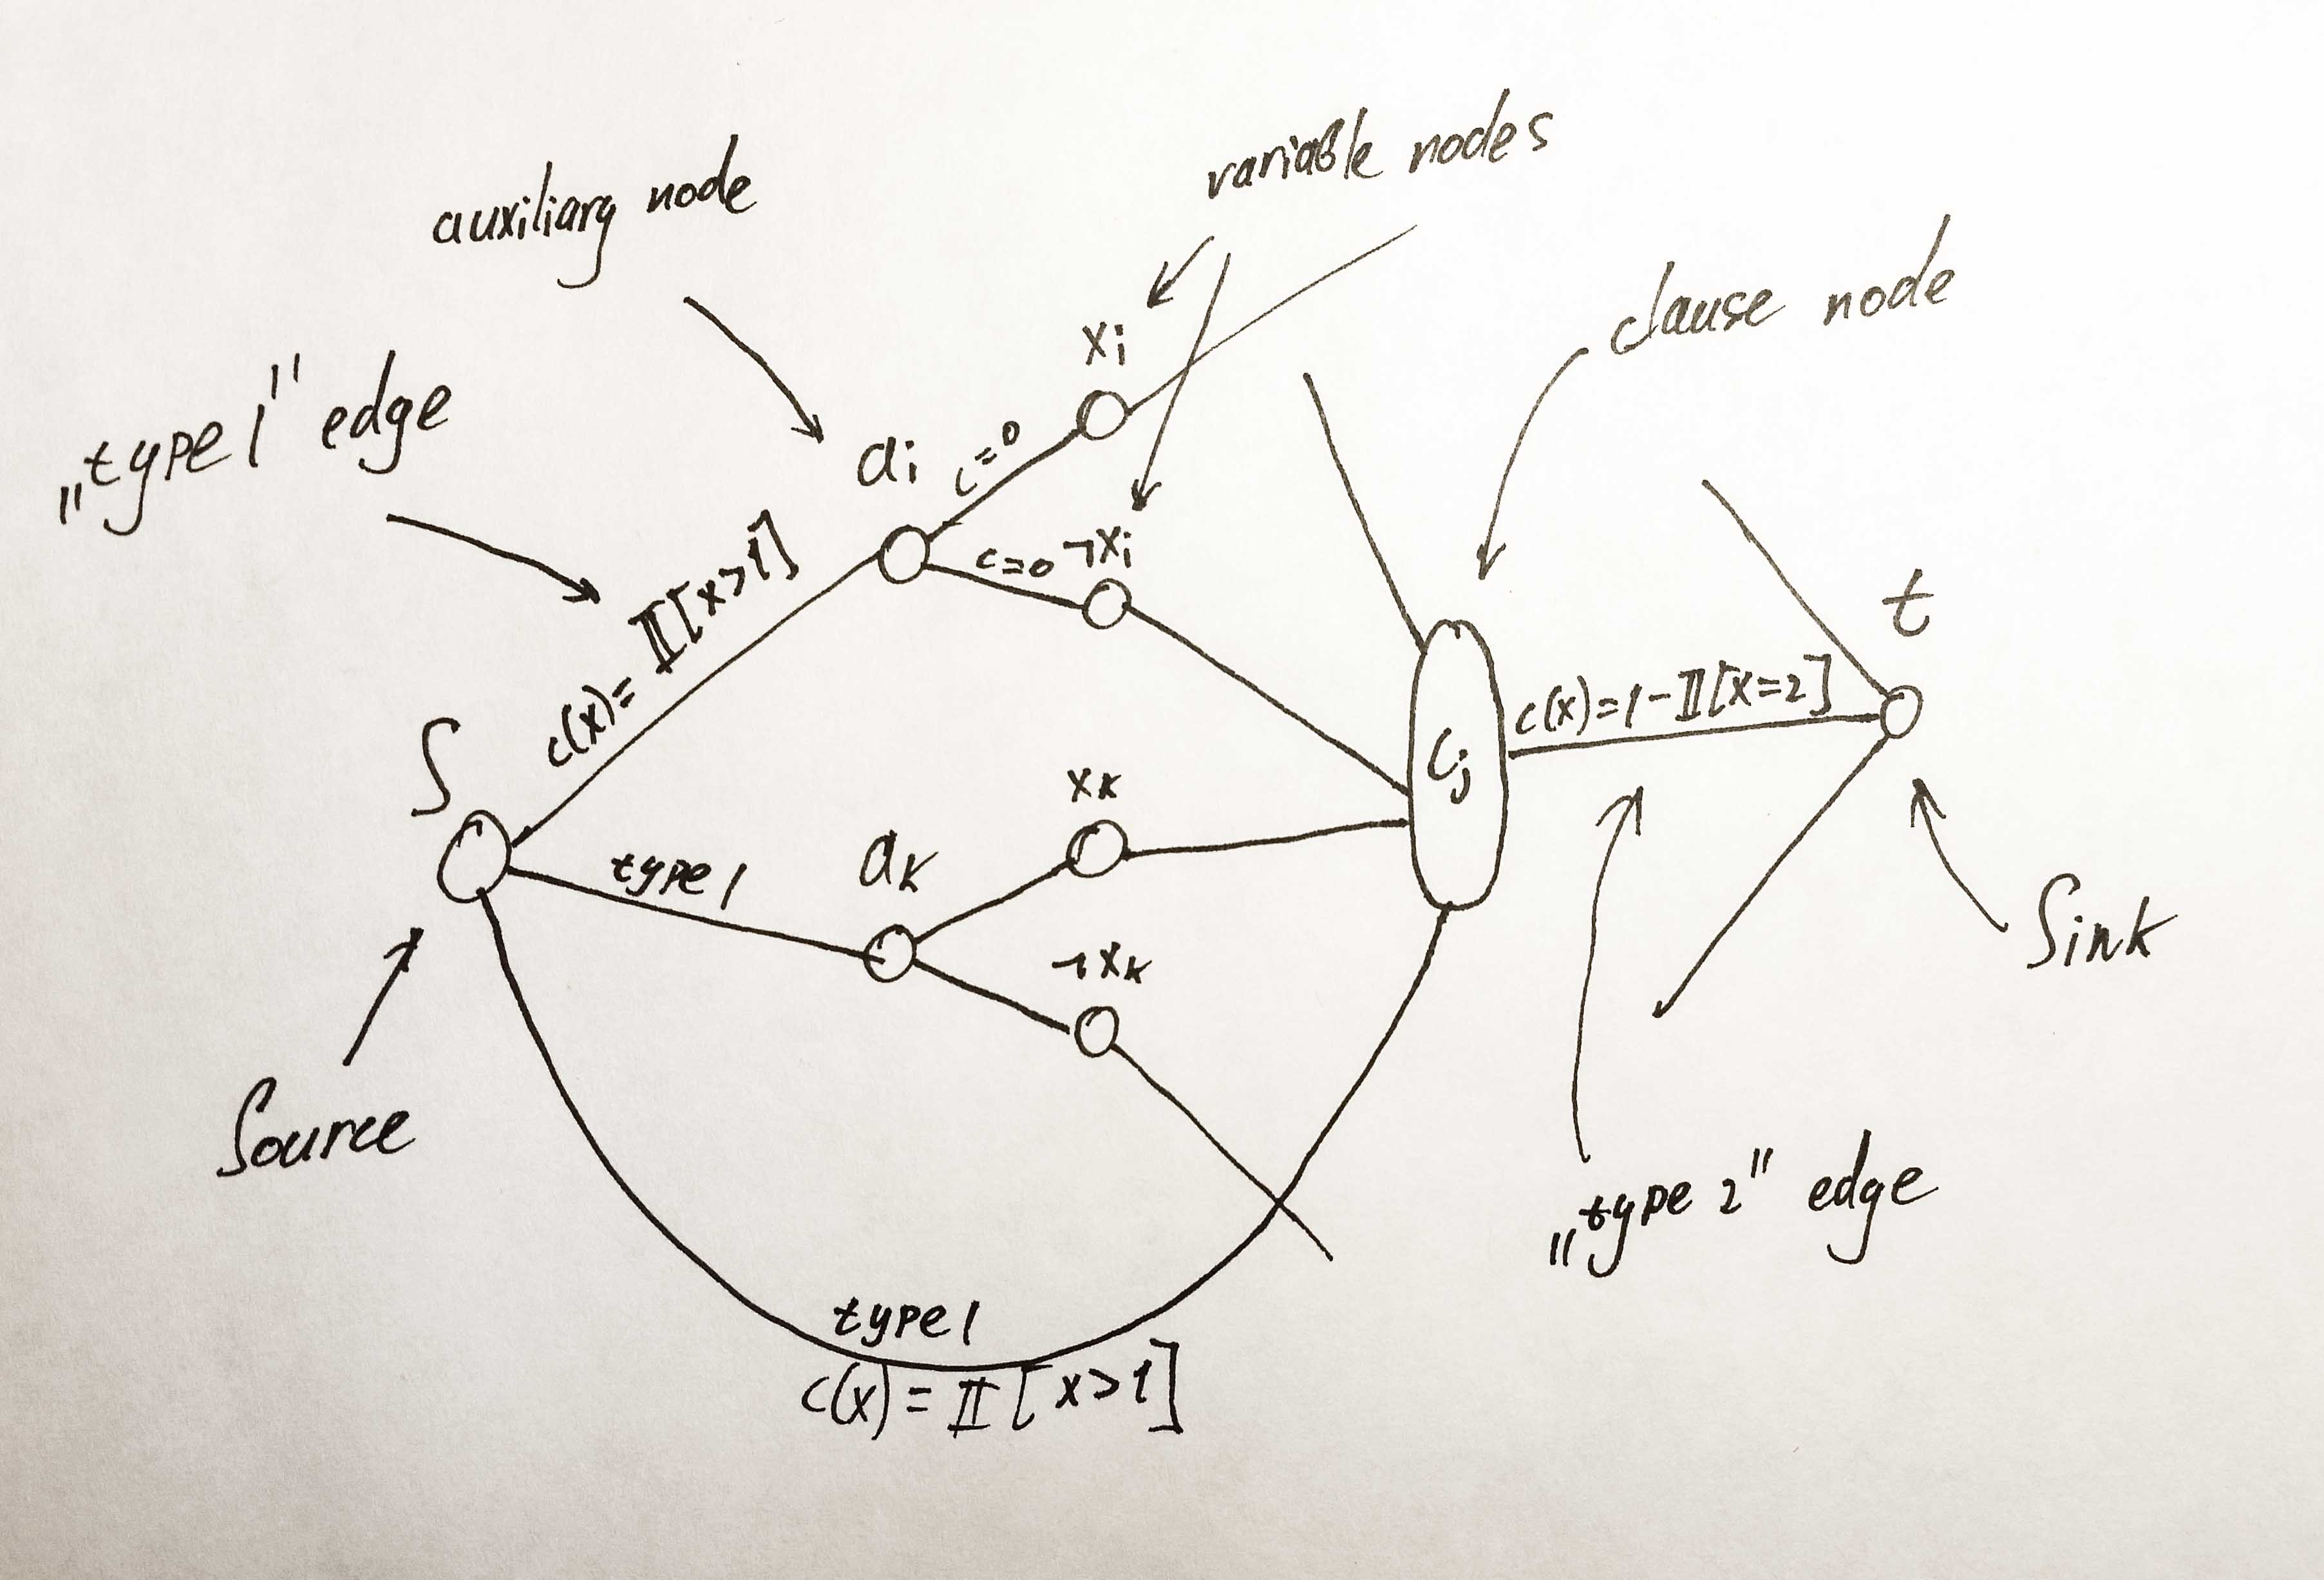
\includegraphics[scale=0.1]{1.jpg}

\uline{\textbf Problem formulation and proof of correctness.} Now, given the graph $G$ above, consider a congestion problem with $m + mn$ agents, where each agent has flow of 1 and has choose a path between $s$ and $t$. 
\bigskip

\uline{\textbf{Lemma}} If original 3SAT is satisfiable, $G$ has a NE of cost 0.

\textit{Proof.} Given a solution to 3SAT, consider the following flow profile. $m$ agents go through type 1 edges between $s$ and $C_j$ then to the variable node $X_i$ such that $x_i$ is true in 3SAT solution (if there are several such nodes, choose arbitrarily), and finally to the sink through the corresponding type 2 edge. 

For remaining $mn$ agents, through type 1 edges send m agents to $X_i$ (to $\neg X_i$) if $x_i$ in the solution of 3SAT is false (is true) for every $i\in[1,n]$.

Now, notice that in such a flow costs on all edges are 0, and so this is an equilibrium (because players incur the cost of 0 and thus cannot improve cost by deviating).

\uline{\textbf{Lemma}} If  $G$ has a NE of cost 0, original 3SAT is satisfiable.

\textit{Proof.}

For cost to be 0, all type 3 edges have to have cost of 0. Assign $x_i$ to be true if connected to it type 3 edge has 0 flow and false if it has flow of $m$ (those are the only possibilities). 

Now take arbitrary clause node $C_j$. Because total cost is 0, it has to be that it has a flow of 1 going through it (if there isn't, there is going to be a type 2 edge from $s$ to $A_i$ that has a flow of more than $m$, which would lead to non-zero cost). We argue that the variable corresponding to the node $X_i$ (or $\neg X_i$) through which this flow goes to the sink is assigned true. Indeed, if it is not so, the corresponding type 2 edge has a flow of at least $m+1$ and hence the cost of 1, which is a contradiction to 0 cost equilibrium. Thus the corresponding to node $C_j$ clause $c_j$ is satisfied by such an assignment.

\uline{\textbf{Theorem}} Finding best NE in a congestion game is NP hard.

\textit{Proof.} Notice that $G$ is polynomial (in m,n) in size and construction time. The statement now follows from previous lemmas: we have demonstrated that we can solve 3SAT by solving corresponding best equilibrium problem, and conversion is polynomial.

